\documentclass[aps,rmp,twocolumn,amsmath,amssymb,nofootinbib,superscriptaddress]{revtex4}

\newcommand{\bra}[1]{\langle#1|}
\newcommand{\ket}[1]{|#1\rangle}
\newcommand{\op}[2]{\hat{\textbf{#1}}_{#2}}
\newcommand{\dagop}[2]{\hat{\textbf{#1}}_{#2}^\dag}
\usepackage[pdftex]{graphicx}
\usepackage{mathrsfs}
\usepackage[colorlinks]{hyperref}
\usepackage[dvipsnames]{xcolor}

\newcommand{\comment}[1]{{\color{blue}{#1}}}

\begin{document}

\bibliographystyle{apsrev}

%
% Title
%

\title{Boson-Sampling with Single Photons: A Roadmap to Post-Classical Computation}

%
% Authors
%

\author{Authors before me}

\author{Peter P. Rohde}
\email[]{dr.rohde@gmail.com}
\homepage{http://www.peterrohde.org}
\affiliation{Centre for Quantum Computation and Intelligent Systems (QCIS), Faculty of Engineering \& Information Technology, University of Technology Sydney, NSW 2007, Australia}

\author{Authors after me}

\date{\today}

\frenchspacing

%
% Abstract
%

\begin{abstract}
Boson-sampling is thus far the most feasible approach for demonstrating the supremacy of quantum computation over classical computation in the near future. We take the view that proof-of-principle demonstration of quantum supremacy is a pressing goal, with enormous implications, and should be considered an utmost priority by the experimental community. Here we strive to outline a roadmap to achieving this elusive goal, examining competing architectures and technologies, and paving the way forward for the first experimental demonstration of post-classical computation. We firstly develop a practical model to compare the performance of boson-samplers and classical simulators. In this model, we find that low-photon-number boson-sampling operating in the current experimental regime (\mbox{$n<10$} photons) could beat present commodity computers with GHz clock-rates only if the overall system efficiency and repetition rate are sufficiently high. Further, we calculate the required efficiency and photon-number to surpass classical computers of different clock-rates using various experimental schemes. Especially, we find that only if both photon-number-resolving detectors and high-speed optical shutters are available, scattershot boson-sampling is feasibly scalable to tens of photons. In order to provide a clear roadmap for boson-sampling, we also review and discuss various state-of-the-art single-photon sources, quantum circuits, and single-photon detectors.
\end{abstract}

\maketitle

\tableofcontents

\section{Introduction} \label{sec:introduction}

Quantum computers are expected to be able to solve certain problems much faster than classical computers \cite{bib:1}, and people have been making unremitting efforts towards them for more than two decades. However, actual quantum computers are presently still in their infancy. Thanks to its simplicity, boson-sampling is expected to be the first specialised quantum computer outperforming classical ones in the near term \cite{bib:2}. More importantly, this would also constitute the strongest evidence yet against a foundational tenet in computer science: the Extended Church-Turing Thesis (ECT), which postulates that all realistic physical systems can be efficiently simulated with a (classical) probabilistic Turing machine. However, the realisation of large-scale boson-samplers still faces many demanding technological challenges, despite being far easier to build than universal quantum computers.

To scale up to a large enough level to exhibit quantum supremacy, the first and most important consideration is the total efficiency of the system, including the generation efficiency of single-photon sources, the coupling and propagation efficiency of the circuit, and the coupling and detection efficiency of single-photon detectors.

In Sec.~\ref{sec:sampling_time}, taking the repetition rate of the sampling system into account, we develop a rigorous and fair model for comparing the performance of boson-samplers and classical simulators. Given a certain classical computer, the regime of quantum supremacy of boson-sampling is specified by a simple continuous curve in the plane of total efficiencies versus photon-numbers. \comment{To our surprise, there is such a (optimal) turning point in this curve where four-photon boson-samplers with repetition rates of 76MHz could beat present commodity computers with GHz clock-rates}. Based upon this, such a computer could only be defeated by \mbox{$20\sim 30$}-photon boson-sampling \cite{bib:2, bib:3}. Furthermore, in Sec.~\ref{sec:exp_schemes}, we calculate the required efficiencies and photon-numbers for different experimental schemes to outperform classical computers of given clock-rates. In particular, we find that both photon-number-resolving detectors and high-speed optical shutters are indispensable to correctly implementing scattershot boson-sampling with tens of photons.

An intact boson-sampler includes three parts (see Fig.~\ref{fig:model}): single-photon sources, passive linear optical circuits, and single-photon detectors. A number of small-scale boson-sampling implementations have been reported in optical waveguides \cite{bib:4, bib:5, bib:6, bib:7, bib:8, bib:9} and fibre beamsplitters \cite{bib:10} using spontaneous parametric down-conversion (SPDC) sources, and fibre-loops \cite{bib:11} with quantum dot (QD) sources. In Sec.~\ref{sec:adv_sources}, we introduce some of the most promising single-photon sources and their recent advances, including SPDC, four-wave mixing (FWM) and QDs. In Sec.~\ref{sec:adv_networks}, we review and discuss some advances in linear optical networks, including optical waveguides, fibre-loops, and fibre beamsplitters. In Sec.~\ref{sec:adv_detectors}, we consider single-photon detectors (SPD), including single-photon avalanche photodiodes (SPAD), superconducting nanowire single-photon detectors (SNSPD) and transition-edge sensors (TES). These three types of detectors represent the most mature, high-speed, and near-unit efficiency respectively.

\begin{figure}[!htb]
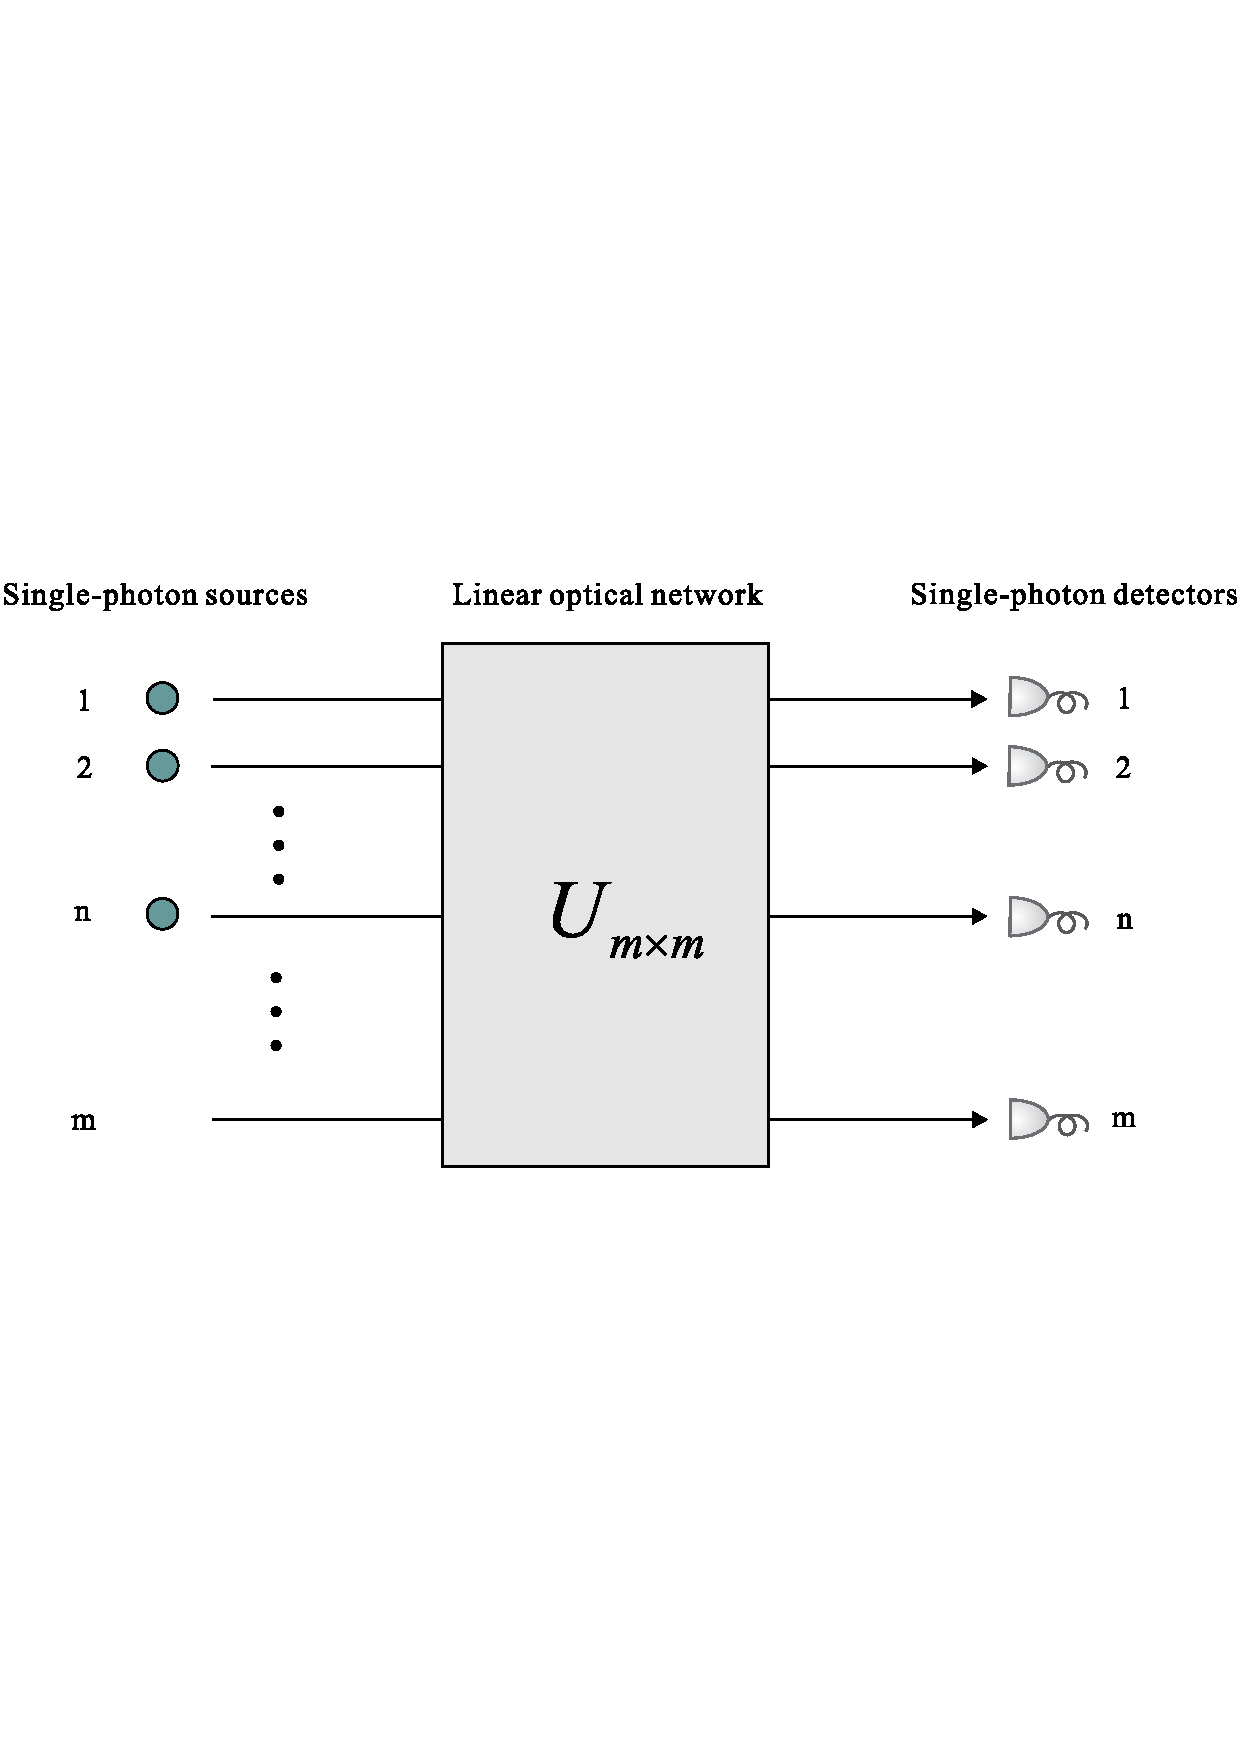
\includegraphics[width=\columnwidth]{model}
\caption{The boson-sampling model. $n$ single photons are injected into an $m$-mode passive linear optical network. The output statistics are then sampled via $m$-fold coincidence photodetection.} \label{fig:model}
\end{figure}

\section{Sampling Time} \label{sec:sampling_time}

In this section, we will first briefly introduce the boson-sampling model and quantum sampling time, then review and discuss classical simulation methods and their respective sampling time, finally performing a quantum versus classical comparison, with the aim of characterising the operating regime for quantum supremacy. We find that with repetition rates of 76MHz, only if the net efficiency of the system is greater than 40\%, four-photon boson-sampling could outperform GHz classical computers. On the other hand, the classical limit may be achieved using a 20-photon boson-sampler with a sampling rate of just 1Hz.

\subsection{Quantum Simulation}

Boson-sampling is a process in which $n$ indistinguishable photons are injected into an $m$-mode linear optical interferometer, characterised by linear optics transformation $U$ (i.e beamsplitters and phase-shifters), and then detected at output ports using photodetectors, as shown in Fig.~\ref{fig:model} \cite{bib:2}. $U$ evolves the photonic creation operators according to,
\begin{align}
\hat{U} \hat{a}^\dag_i \hat{U}^\dag \to \sum_{j=1}^m U_{i,j} \hat{a}^\dag_j,
\end{align}
where $\hat{a}^\dag_i$ is the photon creation operator for the $i$th mode.

Choosing the mode occupation-number configurations as the basis states, the input state can be written as a list of occupation numbers \mbox{$\ket{S}=\ket{s_1,\dots,s_m}$}, where $s_i$ is the number of photons in the $i$th input mode. As photon-number is preserved via linear optics transformations, the output state can be denoted in the same basis, but a superposition of all different output configurations,
\begin{align}
\ket\varphi = \sum_{i=1}^{|\Phi|}\alpha_i \ket{T_i},
\end{align}
where \mbox{$\ket{T_i} = \ket{t_1,\dots,t_m}$}, and with each basis state satisfying
\begin{align}
\sum_{i=1}^m s_i = \sum_{i=1}^m t_i = n \,\,\forall\,\, S,T.
\end{align}
We define $\Phi$ as the set of all photon-number configuration basis vectors. It is not hard to prove that the total number of elements in $\Phi$ is,
\begin{align}
|\Phi|=\binom{m+n-1}{n}.
\end{align}
The amplitude associated with each output basis is given by \cite{bib:2, bib:12},
\begin{align}
\bra{T_i} \Phi(\hat{U}) \ket{S} = \frac{\mathrm{Per}(U_{S,T_i})}{\sqrt{s_1!\dots s_m!t_1!\dots t_m!}},
\end{align}
where $\Phi(U)$ is a homomorphism of $U$, and $U_{S,T_i}$ is an $n\times n$ submatrix of $U$, obtained by taking $s_i$ copies of the $i$th row of $U$, and $t_i$ copies of the $i$th column of $U$. It has been proven that \cite{bib:2, bib:13, bib:14} one will observe a collision (i.e. two or more photons in the same mode) with probability bounded away from 0 only if the number of modes scales as at least $m=O(n^2)$ -- the so-called `bosonic birthday paradox' \cite{???}. In this instance, it suffices to use non-photon-number-resolving detectors, substantially simplifying technological requirements. Thus, throughout this paper we only discuss the `collision-free' situation, i.e. $s_i,t_j=\{0,1\}$.

Consider the practical situation, where we have an imperfect photonic simulator to implement boson-sampling, whose net per-photon efficiency is $\eta$, combining the single-photon generation rate, circuit transmission efficiency, and coupling and detection efficiency (in a linear optics network, all losses can be commuted to the front or back of the circuit, provided all losses are uniform across all modes, allowing us to merge all the individual efficiencies into a single overall efficiency factor). The time required to obtain an $n$-photon coincidence event is,
\begin{align} \label{eq:tau_q}
\tau_q = \frac{1}{\eta^n R}
\end{align}
where $R$ is the effective repetition rate of the quantum boson-sampler, restricted by the choice of single photon source (SPS), the experimental architecture, and the dead-time of the detectors.

\subsection{Classical Simulation}

How can a classical computer simulate this bosonic process, and sample from its exact or approximate probability distribution? A na{\"i}ve brute-force method is to calculate all $|\Phi|$ permanents of the set of submatrices $U_{S,T_i}$, thereby determining the full probability distribution, and then sample from this known distribution. \textbf{However, neither does the boson-sampler know even the approximate probability distribution before enough samples are obtained} \comment{What does that sentence mean?}. Smarter classical algorithms exist to generate correct samples without knowing the entire underlying distribution. For example, using the acceptance-rejection method \cite{bib:15} one can sample an output configuration $\ket{T_i}$ uniformly from the configuration space and a number $u$ from the uniform distribution over $\{0,1\}$, then calculate the permanents of the respective submatrices and compare them to $u$; If \mbox{$u<|\mathrm{Per}(U_{S,T_i})|^2$}, we accept the sample $\ket{T_i}$; If not, it is rejected, and we repeat. Such methods could be successful with probability $O(1)$. One sample only requires calculating one permanent, significantly better than the brute-force method of calculating the entire distribution.

The permanent is a matrix function originating from the permutation symmetry of bosons, similar to the role of determinants for fermions. Na{\"i}ve calculation of the permanent of an $n\times n$ matrix requires $n!$ operations. However, a more efficient classical algorithm developed by Ryser \cite{bib:16} in 1963 requires $O(n^2 2^{n+1})$ operations, which is nonetheless exponential. No general polynomial-time algorithms have been described, in contrast to the clever Gaussian elimination method for calculate matrix determinants. In fact, calculating the permanent was proved to be \#P-complete in 1979 by Valiant \cite{bib:17}. A more intuitive understanding is that the permanent corresponds to counting the number of different matching ways between input state and output state through the interferometer, much like adding Feynman paths \cite{???} to determine quantum amplitudes.

Consequently, for a classical simulator, the time required to acquire a sample using this approach is,
\begin{align} \label{eq:tau_c}
\tau_c \approx \frac{n^2 2^{n+1}}{A},
\end{align}
where $A$ is number of floating-point operations per second (FLOPS) of the classical computer.

\subsection{Threshold}

Comparing the requisite times, we plot the critical photon-number as a function of efficiency $\eta$ for the quantum boson-sampler to beat its classical counterpart, as shown in Fig.~\ref{fig:curves_1}(a). The right part of each line is the area of quantum supremacy. For a given single-photon efficiency, with increasing $n$, the quantum simulator's superiority becomes more prominent. Thus, scaling up the size of boson-sampling is essential to achieving quantum supremacy. But there is an upper limit. Taking \mbox{$\eta=0.4$} as an example, it is impossible to reach quantum supremacy for a classical computer of petaFLOPS by only enlarging the number of single photons. A more convenient approach is to increase the efficiency of the quantum system. As the efficiency increases, the minimum photon-number required to achieve quantum supremacy decreases, simplifying experimental resource requirements.

\begin{figure}[!htb]
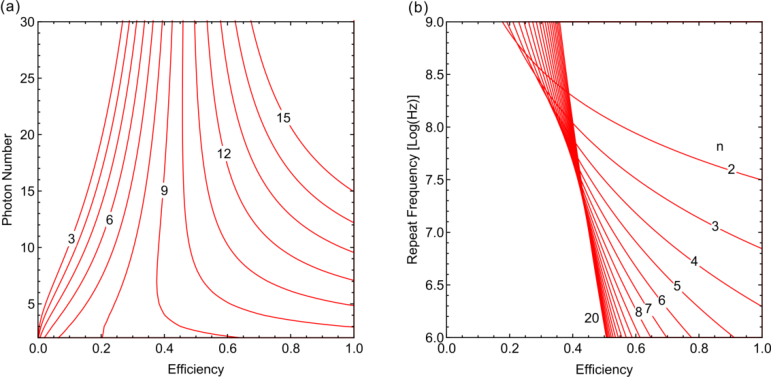
\includegraphics[width=\columnwidth]{curves_1}
\caption{The quantum and classical supremacy of (spatially-encoded) boson-sampling is divided by the red lines, where the top-right region corresponds to quantum supremacy and vice versa. The efficiency denoted on the horizontal axis is the overall system efficiency. (a) $R=76$MHz. The numbers 3, 6, etc. in the lines refer to $10^3\mathrm{FLOPS}$, $10^6\mathrm{FLOPS}$ etc. of the classical simulator. (b) $A=10^9\mathrm{Hz}$. The numbers 2, 3, etc. in the lines denote photon-number.} \label{fig:curves_1}
\end{figure}

The repetition rate $R$ is another important factor affecting the performance of quantum simulators that we must consider in practical experiments. If $\eta^n$ is taken as the post-selection success probability of a single trial, then \mbox{$\eta^n R$} indicates how many successful runs we can implement per second. For example, to beat a gigaFLOPS classical computer, four-photon boson-sampling with $R=76\mathrm{MHz}$ ($R$ vs $A$) is sufficient if the total efficiency is \mbox{$\eta=0.4$}. As shown in Fig.~\ref{fig:curves_1}(b), however, \mbox{$\eta=0.2$} and \mbox{$n=2$} is sufficient if the repetition rate increases to 1GHz. In other words, by increasing the repetition rate, the efficiency and photon-number requirements are relaxed. However, we cannot increase the repetition rate indefinitely. It is restricted by the pulse rate of the SPS, experimental architecture, and dead-time of the detectors. In the next section we discuss the impact of the choice of experimental architecture.

Here we must point out two things. First, Ryser's algorithm is actually not faster than using the original formula to calculate the matrix permanent when photon number is small (\mbox{$n<6\sim 7$}). Thus the above conditions may be not tight. For example, the efficiency must be larger than $\sim 0.6$ if two- (four)-photon boson-sampling with a repetition rate of 1GHz (76MHz) is expected to beat a gigaFLOPS classical computer. 

Why then should we nonetheless scale up to more photons (\mbox{$n=20\sim 30$}), even though boson-sampling with relatively few photons could beat current prevailing personal computers in realistic experimental regimes? One reason is that no finite experiment can make a decisive conclusion about the ECT, since it is a conjecture about the asymptotic limit. In the field of computational complexity, the significance of boson-sampling rests largely on its exponentially faster sampling speed than that of classical simulators, rather than certain times of specific triumphs in the competitions between quantum and classical computers. Thus, through upscaling we can make stronger statements about asymptotic behaviour (albeit never a completely conclusive one). Another cause is that people have not physically constructed relatively large multi-photon interferometers yet. The theory of boson-sampling still faces the risk of failure and quantum devices may break down with more photons. Finally, although no practical uses for boson-sampling have been described, it is entirely plausible that useful applications may be found in the future. Were that the case, scaling up boson-sampling experiments would similarly scale up the size of the problems it could solve.

\section{Experimental Schemes} \label{sec:exp_schemes}

\subsection{Spatial Encoding Architecture}

A fully spatially-encoded scheme is one whereby the circuit itself does not consume any time resources (beyond the propagation time from the input to the output time of the circuit, which is fixed). This includes optical waveguides, fused fibre couplers and bulk-optics circuits, as shown in Fig.~\ref{fig:space_encoding}. The time required for this scheme is the same as Eq.~\ref{eq:tau_q}.

\begin{figure}[!htb]
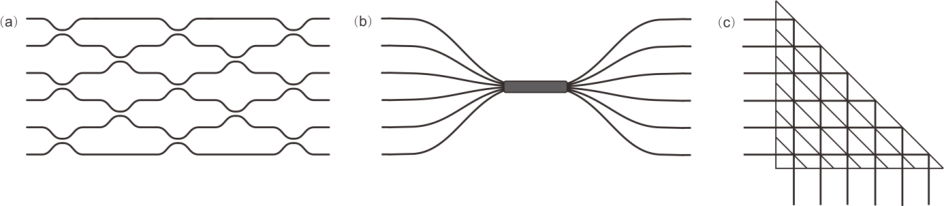
\includegraphics[width=\columnwidth]{space_encoding}
\caption{Spatially-encoded optical circuits: (a) optical waveguide; (b) fused fibre coupler; and, (c) bulk-optics.} \label{fig:space_encoding}
\end{figure}

It was proven by Reck et al. \cite{bib:18} that an arbitrary $m$-mode linear optical network can be efficiently constructed using $O(m^2)$ linear optical elements (i.e. beamsplitters and phase-shifters). This can be reduced to $O(mn)$ in the case of boson-sampling, where there are $n$ photons in $m$ modes. Although `efficient', this scaling implies that constructing a network with hundreds of modes with discrete elements, one probably needs several room-sized optical tables, inevitably suffering from severe air turbulence and mechanical instability. For perfect quantum interference, photons should arrive at the points of interference simultaneously and be perfectly mode-matched (to be discussed in more detail in Sec.~\ref{sec:fidelity_of_devices}), which means all of the thousands of optical elements must be carefully simultaneously aligned. More integrated and stable alternatives are of pressing importance. In fact, all initial demonstrations of boson-sampling were based on integrated optical circuits including, waveguides based on direct laser writing techniques \cite{bib:4, bib:5, bib:6} and fused fibre couplers \cite{bib:10}.

\subsection{Time-Bin Encoding Architecture}

An alternative scheme fully employs time-bin encoding to construct the interferometer network, which was proposed \cite{bib:19} in 2014 and first demonstrated \cite{bib:11} in 2016. The main idea is to utilise the temporal degree of freedom, by applying a mapping from spatial modes to time-bins. This scheme has fixed experimental complexity and only needs one high repetition rate SPS, one time-resolved detector and one dynamic beamsplitter, which makes it much easier to align the experimental setup since there is only a single point of interference. The architecture is shown in Fig.~\ref{fig:loop_arch}.

\begin{figure}[!htb]
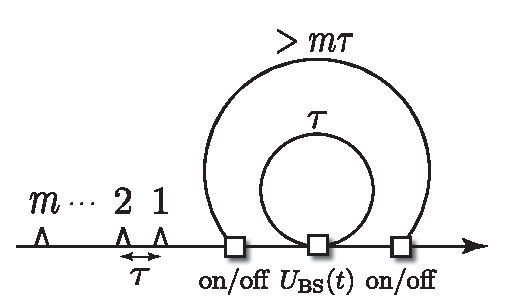
\includegraphics[width=\columnwidth]{loop_arch}
\caption{The fibre-loop scheme for boson-sampling. A pulse-train of photons in $m$ time-bins defines the input state, with time-bin separation $\tau$. The pulse-train is coupled into and out of the outer loop using two outer dynamic switches. The inner loop of length $\tau$ allows neighbouring time-bins to interfere at the central dynamic switch. The outer two switches need only switch between being completely reflective and completely transmissive, whereas the inner switch must be able to tune to any beamsplitter reflectivity. The only component that scales with the size of the interferometer is the length of the outer loop, which must be long enough to contain the entire pulse-train, $>m\tau$.} \label{fig:loop_arch}
\end{figure}

In this design, a sequence of single photons is injected and interference with one other through the time delay and fibre beamsplitter. As in Fig.~\ref{fig:loop_arch}, a small fibre loop of round-trip time \mbox{$\tau=1/R$} acts as the time delay, where the node is a dynamic beam splitter for interference. The small loop is embedded in a large fibre loop of travelling time $>m\tau$, which is used to return the `photon pulse-train' back for next round of interference. These two embedding fibre loops together fully construct the interference network that encodes only in the temporal degree of freedom. According to Reck's result, one needs $O(m^2)$ beamsplitters to construct an arbitrary \mbox{$m\times m$} interferometer. For a with $m$ time bins, the beamsplitter works $m$ times in each round trip. So $m$ round trips are required to implement an arbitrary  unitary transformation. After $m$ loops of evolution, the photons are all coupled out of the loop for time-resolved coincidence measurements.

As described above, the circuit itself consumes time resources $m^2\tau$, thus the effective repetition rate is,
\begin{align}
\frac{1}{m^2\tau}=\frac{R'}{m^2},
\end{align}
where $R'$ is the repetition frequency of the photonic time-bins. We use it instead of $R$ in Eq.~\ref{eq:tau_q} and obtain,
\begin{align}
\tau_t = \frac{m^2}{\eta^n R'}.
\end{align}
Comparing $\tau_t$ with $\tau_c$ and following the same way for original boson-sampling in Sec.~\ref{sec:sampling_time}, we plot the critical photon-number to reach quantum supremacy as a function of $\eta$ for the time-bin encoding scheme.

We see that the boundary lines in Fig.~\ref{fig:curves_2} move to the right relative to Fig.~\ref{fig:curves_1}(a), in the case of utilising spatial encoding. For example, to beat a classical computer of gigaFLOPS, the minimum required photon number increases to 9 if we employ time-bin encoding. This is because, for temporal encoding, there is only one spatial mode so that all the $m^2$ operations to realise the unitary transformation can only be extended in the temporal degree of freedom. Thus, its scalability is forced to be more dependent on the repetition rate of the SPS and the dead-time of the single-photon detector.

\begin{figure}[!htb]
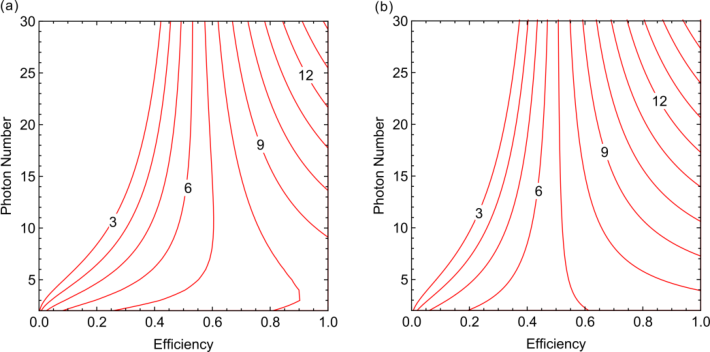
\includegraphics[width=\columnwidth]{curves_2}
\caption{The quantum and classical supremacy of (a) temporal-encoding, and (b) hybrid-encoding boson-sampling, is divided by the red line, where quantum supremacy is in the top-right region, and vice versa. The numbers 3, 6, etc. in the line refer to $10^3$FLOPS, $10^6$FLOPS etc. of classical computers respectively. The efficiency denoted on the horizontal axis is the overall system efficiency. Given the magnitude of the coupling strength, a single step including a beam splitter operation and phase-shifting operation takes \mbox{$\tau\sim0.3\mu\mathrm{s}$} \cite{bib:20}. Effective repeat frequency (a) \mbox{$R'=1/(13\mathrm{ns}\cdot 10^4)$}, (b) \mbox{$R'=1/(0.3\mu\mathrm{s}\cdot n^2).$}} \label{fig:curves_2}
\end{figure}

\subsection{Hybrid Encoding Architecture}

The unitary network can also be encoded into a hybrid architecture -- partially spatial and partially temporal. Recently, Peropadre et al. \cite{bib:20} proposed such a hybrid scheme based on a superconducting device, named `microwave boson-sampling'. They pointed out that, the three fundamental steps of boson-sampling -- i.e. preparation of single-photon states, unitary transformations, and photodetection -- can all be realised using microwave photons with high fidelity (shown in Fig.~\ref{fig:microwave}). For $m$-mode boson-sampling, one needs $m$ storage resonators in total, where microwave photons are produced and stored. And between every pair of adjacent storage resonators there is a superconducting ring to tune the coupling. Each storage resonator has a corresponding X-mon qubit, which plays an essential role in preparation, phase-shifting and measurement. At the other side of the X-mon qubit, a low-Q (measurement) resonator is coupled to implement non-demolition measurement.

\begin{figure}[!htb]
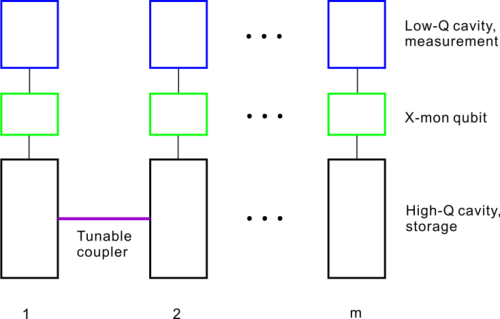
\includegraphics[width=\columnwidth]{microwave}
\caption{Hybrid-encoding (microwave) boson-sampling proposed in \cite{bib:20}. The X-mon qubit is capacitively coupled to the storage and measurement cavities. The tuneable coupler between adjacent storage cavities is a superconducting ring intersected by a Josephson junction.} \label{fig:microwave}
\end{figure}

Compared to fabricating a unitary network in waveguides, the spatial degree of freedom in the transverse axis is retained as there are $m$ storage resonators and auxiliary qubits in microwave boson-sampling. But the longitudinal spatial modes are replaced by $m$ controlled temporal steps. Suppose a single step including a beamsplitter operation and phase-shift operation takes time $\tau_m$, so the total operational time for an \mbox{$m\times m$} unitary transformation is $\tau_m m$ \comment{Shouldn't this be $m^2$?}. Taking the reciprocal of the total operational time as the effective repeat frequency, we obtain the formula for $\tau_q$ for this scheme. Comparing with $\tau_c$, we plot the supremacy boundary for microwave boson-sampling, shown in Fig.~\ref{fig:curves_2}(b).

From the perspective of the encoding scheme, the sampling speed (unitary transformation) of microwave a boson-sampler is much slower than that of spatially-encoding boson-samplers. As showed in Fig.~\ref{fig:curves_2}, to beat the same advanced classical computer, we actually need higher system efficiency or a larger number of photons if the microwave scheme is utilised. However, the advantage of the superconducting platform exactly lies in its marvelously high fidelities ($>0.90$) of generation and measurement processes \cite{bib:21}, to which no ordinary optical boson-sampler is comparable. Though with high processing speed, the effective repeat frequency of a spatially-encoded optical boson-sampler is greatly reduced by post-selection due to the limited collection and detection efficiency. \comment{This doesn't make sense to me - explain it better}

\subsection{Lossy Boson-Sampling}

In real-world experiments, photons are inevitably subject to loss and other errors, making it sample from an erroneous distribution rather than the desired boson-sampling distribution. As boson-sampling only comprises passive optical elements, it is not universal and there are no known fault tolerance or error-correction schemes. From the beginning, Aaronson and Arkhipov 
cite{bib:2} have already noted this problem. And in their original paper introducing boson-sampling, proved that boson-sampling is classically hard even if sampling from an approximate distribution with multiplicative error. Furthermore, several follow-up works have discussed the effect of realistic experimental imperfections in more detail, such as losses \cite{bib:22}, mode-mismatch due to calibration errors within the linear optical network \cite{bib:23, bib:24}, and photon distinguishability \cite{bib:25, bib:26, bib:27, bib:28, bib:29, bib:30}.

It was shown that the hardness remains in the same complexity when the average fidelity per optical element of the unitary network scales as \mbox{$1-O(1/n^2)$}. In the presence of varying degrees of photon distinguishability, the probability of each sample is related to an immanent, a more general matrix function than permanents and determinants, conjectured to be as computationally hard as the permanent in general \cite{bib:31, bib:32}.

To deal with photon loss due to sub-unity transmittance within the circuit and inefficient detection, post-selection, which discards samples with lost photons, is usually adopted in experiments. However, assuming that on average each photon has a constant probability to finally trigger a detector at the output, the experimental runtime overhead arising from post-selection will increase exponentially with the number of photons in the system.

Recently, Aaronson and Brod \cite{bib:33} demonstrated that if $O(1)$ photons are lost at the input (i.e. $k$ out of \mbox{$n+k$}), the probability of each output configuration is given by,
\begin{align}
\mathrm{Pr}(T) = \frac{1}{|\Lambda_{n+k,n}|} \sum_{s\in m,n+k,n} |\mathrm{Per}(U_{S,T})|^2.
\end{align}
\comment{Need to define $\Lambda$ and meaning of $s\in m,n+k,n$.}

It was also proved that calculating $\mathrm{Pr}(U_{S,T})$ is as least as hard as calculating the permanent of an \mbox{$m\times n$} submatrix of a Harr-random matrix. Let us introduce a modification of $\tau_q$ and $\tau_c$ in the context of boson-sampling with lost photons. The average sampling interval $\tau_q$ is obtained by replacing the probability of detecting $n$ photons in coincidence, $\eta^n$, in Eq.~\ref{eq:tau_q} with,
\begin{align}
P(n,n_\mathrm{los}) = \eta^n(1-\eta)^{n_\mathrm{lost}}\binom{n+n_
\mathrm{lost}}{n_\mathrm{lost}},
\end{align}
where $n$ is the number of photons after loss, and $n_\mathrm{lost}$ is the number of lost photons. So we have,
\begin{align}
\tau_q = \frac{1}{\eta^n(1-\eta)^{n_\mathrm{lost}}\binom{n+n_
\mathrm{lost}}{n_\mathrm{lost}}R}.
\end{align}

Because \emph{Theorem 1} in \cite{bib:33} states that boson-sampling with a constant number of lost photons is (at least) as hard as ideal boson-sampling, then for a classical simulator, Eq.~\ref{eq:tau_q} can still be applied to boson-sampling with lost photons whose photon number after loss is $n$.

Provided the repeat frequency of the quantum system is 76MHz and the clock speed of the classical computer is 1GHz, in Fig.~\ref{fig:curve_hybrid} we plot the minimum required number of photons after loss to achieve quantum supremacy against the increasing total efficiency of the quantum boson-sampler.

\begin{figure}[!htb]
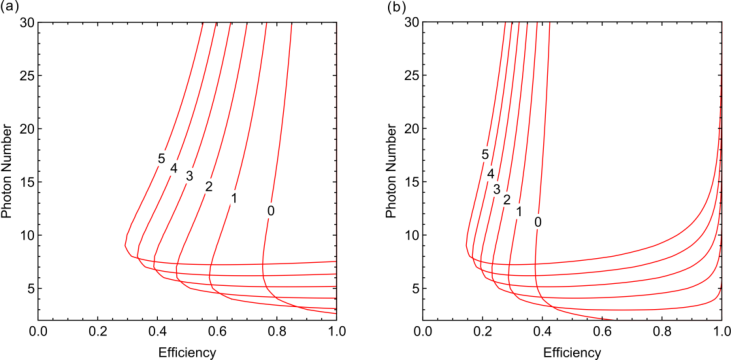
\includegraphics[width=\columnwidth]{curves_loss}
\caption{The quantum and classical supremacy of boson-sampling with lost photons is separated by the red line, where the top-right side corresponds to the quantum regime and vice versa. Here the clock speed of the classical computer is gigaFLOPS, i.e $10^9$FLOPS. The efficiency denoted on the horizontal axis is the overall system efficiency. The numbers 0, 1, 2 \emph{etc.} in the line refer to the number of lost photons, $n_\mathrm{lost}$. The detection efficiency: (a) \mbox{$\eta_d=0.5$} (b) \mbox{$\eta_d=1$}. \comment{(Why does the curve have the change in direction?})} \label{fig:curve_hybrid}
\end{figure}

From right to left, the lines respectively refer to no lost photons, one lost photon, and so on. It is shown that when the efficiency is lower than $\sim 0.4$, theoretically, a quantum sampler implementing standard boson-sampling cannot win the game no matter how large it scales in size. However, by employing the scheme of boson-sampling with lost photons, a quantum sampler of $\sim 0.3$ total efficiency can beat the classical competitor if 5 photons remain after loss and another extra photon was injected but lost. Our result agrees with Rohde's theory \cite{bib:22} that quantum superiority can be retained by injecting extra photons to compensate for loss in the quantum device.

\subsection{Scattershot Boson-Sampling}

The brightness of $n$ photons will decay exponentially as $p^n$ if each SPS has efficiency $p$. For current mature heralded SPSs based on spontaneous parametric down-conversion (SPDC), one solution is to introduce more SPDC sources and make $p$ approach unity by the technique of multiplexing \cite{bib:34}. For boson-sampling, there is an even simpler method known as `scattershot' boson-sampling (SBS) \cite{bib:35, bib:36}, which allows us to perform an identically hard computation without deterministic SPSs or multiplexers. The core idea is to run $m$ SPDCs simultaneously, and post-select the instances where $n$ heralded detectors are triggered, regardless of which detectors click. SBS seems something of a `double sampling' problem, which can be decomposed into uniform sampling at the input state, followed by ordinary boson-sampling. But each single sample is an instance of original boson-sampling with different input states. In fact, Aaronson \cite{bib:35} and Lund \cite{bib:36} pointed out that SBS remains in the same computational complexity class. The first 3-photon experiment has been implemented with 6 equivalent SPDC sources in a 13-mode circuit \cite{bib:38}. The model is shown in Fig.~\ref{fig:scattershot_model}.

\begin{figure}[!htb]
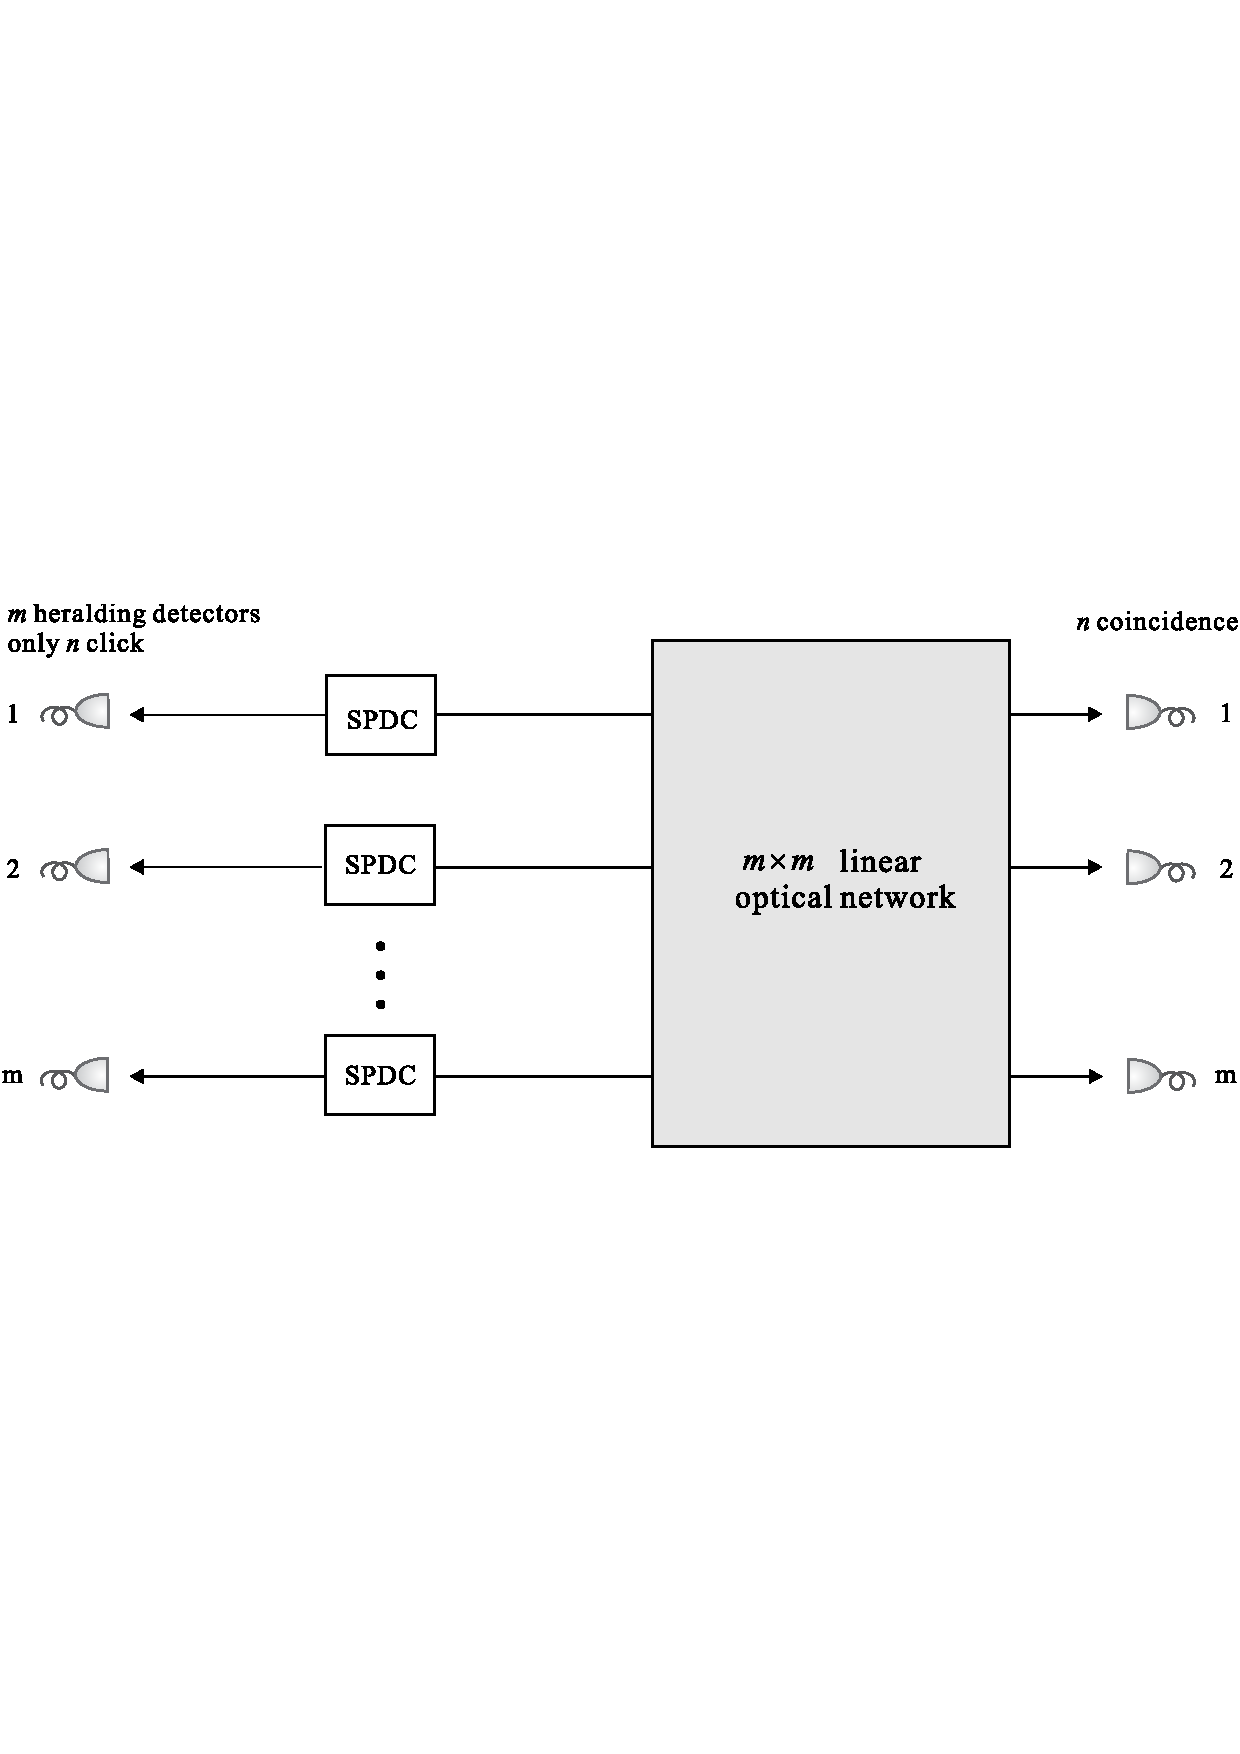
\includegraphics[width=\columnwidth]{scattershot_model}
\caption{The scheme for scattershot boson-sampling \cite{bib:36}. For an \mbox{$m\times m$}-mode interferometer, there are $m$ pairs of SPDCs, of which only $n$ generate single photons at a time.} \label{fig:scattershot_model}
\end{figure}

It is well-known that the two-mode squeezed state via SPDC has the form
\begin{align}
\ket\psi_\mathrm{SPDC} = \sqrt{1-\chi^2}\sum_{N=0}^\infty \ket{N,N},
\end{align}
where $N$ is photon-number and $\chi$ is the squeezing parameter, related to the nonlinearity of the crystal, the pump amplitude and the crystal length. Thus the SPS efficiency is $p=\chi^2(1-\chi^2)$. The model of SBS is illustrated in Fig.~\ref{fig:scattershot_model}. There are in total $\binom{m}{n}$ combinations of different acceptable input configurations, and the generation probability of $n$ single photons is therefore promoted to,
\begin{align}
P(n) = \binom{m}{n} \chi^{2n}(1-\chi^2)^{n^2}.
\end{align}

When \mbox{$\chi=1/\sqrt{n+1}$} or \mbox{$p=n/(n+1)^2$} \cite{bib:36}, the generation probability $P(n)$ can be maximised to,
\begin{align}
P_\mathrm{max}(n) = \frac{1}{e\sqrt{2\pi n}}.
\end{align}
This only incurs an $O(\sqrt{n})$ overhead to the initial state preparation compared to deterministic SPSs. Then given there are in total $2m$ detectors in SBS, we can express $\tau_q$ for scattershot boson-sampling as,
\begin{align}
t_{q(\mathrm{SBS})} = \frac{P_\mathrm{max}(n)}{\eta_t^n\eta_d^n R},
\end{align}
where $\eta_t$ is the detection efficiency of the triggering detector, and $\eta_d$ is the net efficiency to detect a photon after the optical network.

As pointed out in Sec.~\ref{sec:sampling_time}, the only thing we care about in the competition of quantum boson-samplers versus classical simulators is who would be the first to produce a legitimate sample from the permanent-related probability distribution. And in the context of no a priori knowledge about which input configuration would be picked in the experiment, to simulate SBS, a classical computer can obtain a legitimate sample just by simulating ordinary boson-sampling with deterministic input states. Thus, we follow the same $t_c$ in Eq.~\ref{eq:tau_c} for SBS, which does not need to be multiplied by a combinatorial factor at all as in \cite{bib:37}.

By comparing $\tau_q$ and $\tau_c$, in Fig.~\ref{fig:curve_scattershot} we plot the supremacy boundaries for SBS using nondeterministic SPS via SPDC. We can see that, with the help of the number of different combinations, SPDC survives and SBS is a feasible approach to beating advanced classical competitors. However, in order to scale SBS to the interesting regime of $20\sim 30$ photons, other challenges remain challenging. First, SBS requires $n^2$ SPDC sources, quadratically more than the usual $n$. And a larger-depth optical network is required to fully implement an $m\times m$ unitary matrix, rather than in original boson-sampling, with a fixed number of $n$ input modes, it can be simplified to an $m\times n$ matrix. Besides, as twice the number of photodetectors will be employed, to assure a certain sample rate, the requirement of detection efficiency imposed on photodetectors of SBS would be higher. Comparing Fig.~\ref{curves_1} and Fig.~\ref{fig:curve_scattershot}, we see that, to beat a classical computer, SBS should either scale to a large size or require the quantum device to have a higher total efficiency with respect to ordinary boson-sampling.

\begin{figure}[!htb]
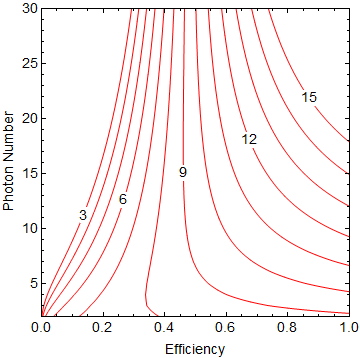
\includegraphics[width=0.5\columnwidth]{curve_scattershot}
\caption{The quantum and classical supremacy of scattershot boson-sampling is separated by the red line, where the top-right region belongs to quantum supremacy and vice versa. The numbers 3, 6, etc. on the lines refer to $10^3$FLOPS, $10^6$FLOPS etc. of classical computers respectively. The efficiency denoted on the horizontal axis is the overall system efficiency except the preparation efficiency of the source, whereby the preparation efficiency of $n$ sources is substituted with $1/\sqrt{2\pi n}$ \cite{bib:36}.} \label{fig:curve_scattershot}
\end{figure}

%\begin{figure}[!htb]
%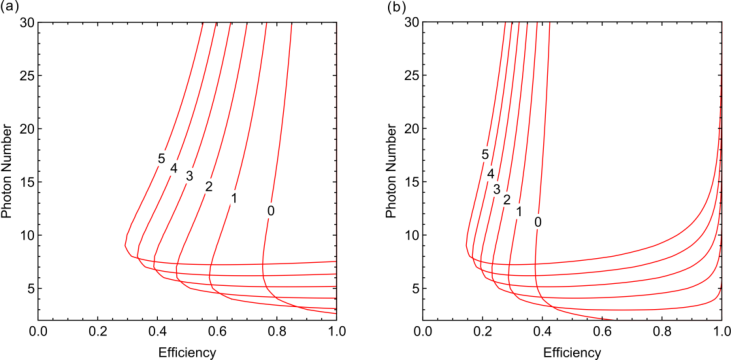
\includegraphics[width=\columnwidth]{lossy}
%\caption{???} \label{fig:lossy}
%\end{figure}


\section{Fidelity of Boson-Sampling Devices} \label{sec:fidelity_of_devices}

Thus far, we have considered sampling rates as the benchmark for performing a classical versus quantum comparison for supremacy. However, it is not only the rate at which samples are be obtained that is of importance. Just as important is the quality of the samples -- are they correct, and do they actually correspond to what would come of a true boson-sampler?

Our analysis thus far has taken loss into consideration as a dominant form of error. As we have seen, this type of error manifests itself in the overall efficiency of the system, and is easily modelled as such. In this section we consider other realistic errors arising in experimental boson-sampling devices and how they impact operation. We give special attention to spatio-temporal errors, whereby imperfections result in degradation of photon indistinguishability, thereby undermining correct multi-photon interference. This analysis encompasses, amongst others, the following prominent error mechanisms in realistic experimental scenarios:
\begin{itemize}
\item Source time-jitter: This is caused by classical uncertainty in the preparation time of photons' wavepackets, yielding a state which is mixed in the temporal degree of freedom. This could arise, for example, from the finite time-resolution of the heralding detector in a heralded SPDC source. 
\item Source spectral impurity: The equivalent effect as before, but in the spectral domain. This is known to be particularly problematic when employing heralded SPDC sources. If an SPDC photon-pair is not perfectly spectrally separable, heralding one mode projects the other mode onto a spectrally mixed state.
\item Mode-mismatch: When photons interfering at a beamsplitter are not perfectly indistinguishable, quantum interference is reduced. This arises whenever optical modes are not perfectly aligned upon interfering at a beamsplitter. In the limit of completely distinguishable photons, boson-samplers obey classical statistics, which are computationally easy to simulate.
\end{itemize}

To model the above, we must first employ a representation for photons, which accommodates their spatio-temporal structure. Ordinarily, we represent photons as the photon creation operator acting on the vacuum state, \mbox{$\ket{1}=\hat{a}^\dag\ket{0}$}. This is appropriate when dealing with indistinguishable photons. However, photons have rich spatio-temporal structure, and in these degrees of freedom photons are never perfectly indistinguishable. To capture this, we replace photon creation operators with mode operators \cite{bib:RohdeMauerer}, that represent photons in these additional degrees of freedom. In the temporal degree of freedom, for example,
\begin{align}
\hat{A}^\dag_\psi = \int_{-\infty}^\infty \psi(t) \hat{a}^\dag(t) \,dt.
\end{align}
Here $\psi$ is the temporal distribution function (TDF) of the photon, and $\hat{a}^\dag(t)$ is the time-specific creation operator. $\psi$ is normalised, such that,
\begin{align}
\int_{-\infty}^\infty |\psi(t)|^2 \, dt = 1.
\end{align}
The Fourier transform gives us the spectral distribution function. Then, a single-photon state with associated TDF $\psi$, is given by,
\begin{align}
\ket{1_\psi} = \hat{A}^\dag_\psi \ket{0}.
\end{align}
This can be logically generalised into other degrees of freedom, such as the spatial degrees of freedom. For example, to capture both temporal and $x$-$y$ spatial degrees of freedom, we could use the representation,
\begin{align}
\hat{A}^\dag_\psi = \int_{-\infty}^\infty \int_{-\infty}^\infty \int_{-\infty}^\infty \psi(t,x,y) \hat{a}^\dag(t,x,y) \, dt\, dx\, dy.
\end{align}

The overlap between two single-photon states characterised by distinct TDFs is simply,
\begin{align}
\langle 1_\psi | 1_\phi \rangle &= \bra{0} \hat{A}_{\psi} \hat{A}^\dag_{\phi} \ket{0} \nonumber \\
&= \int_{-\infty}^\infty \int_{-\infty}^\infty \psi(t)^*\phi(t') \langle t|t'\rangle \, dt \, dt' \nonumber \\
&= \int_{-\infty}^\infty \int_{-\infty}^\infty \psi(t)^*\phi(t') \delta(t-t')\,dt \, dt' \nonumber \\
&= \int_{-\infty}^\infty \psi(t)^*\phi(t) \,dt.
\end{align}

If we choose an orthonormal basis of TDFs, an arbitrary photon may be decomposed into a linear combination of the associated basis mode operators. Let us define such a basis as $\{\xi\}$. Let $\xi_0$ be the `desired' spatio-temporal mode. Because of the orthonormality,
\begin{align}
\bra{0} \hat{A}_{\xi_i} \hat{A}^\dag_{\xi_j} \ket{0} = \delta_{i,j},
\end{align}
we define our mode operators as,
\begin{align}
\hat{A}^\dag_{\psi_i} = \alpha \hat{A}^\dag_{\xi_0} + \sqrt{1-\alpha^2} \hat{A}^\dag_{\xi_i}.
\end{align}
That is, each input photon has an amplitude overlap of $\alpha$ with every other, via the $\xi_0$ component of the TDF. Thus, $\alpha$ characterises the degree of photon distinguishability in the system.

Exactly the same argument applies to incoherent processes, such as time-jitter, except that rather than being a coherent superposition of different spatio-temporal modes, the density operator would be a classical mixture of the different terms,

Then the fidelity of a single-photon input (i.e its overlap with all other photons) is,
\begin{align}
F_\mathrm{in} = |\alpha|^2.
\end{align}
The fidelity of the entire $n$-photon input state is then,
\begin{align}
F_\mathrm{total} &= {F_\mathrm{in}}^n \nonumber \\
&= |\alpha|^{2n}.
\end{align}
This can be interpreted as the probability that, upon measurement, we have projected onto the desired spatio-temporal mode.

Since the fidelity between two states is invariant under a common unitary evolution,
\begin{align}
F(\hat\rho_1,\hat\rho_2) = F(\hat{U}\hat\rho_1\hat{U}^\dag, \hat{U}\hat\rho_2\hat{U}^\dag),
\end{align}
the output fidelity is the same as the input fidelity, \mbox{$F_\mathrm{out} = F_\mathrm{total}$}. The output fidelity has a direct operational interpretation, as the probability that a given sample was taken from a boson-sampling distribution (as opposed to some other erroneous distribution).

The relationship between the single-photon input and net output fidelities are illustrated in Fig.~\ref{fig:fidelity}. Based on this, to achieve an output fidelity of \mbox{$F_\mathrm{out} = 0.9$} (i.e 90\% confidence that a given sample is a legitimate boson-sampling sample) requires single-photon input fidelities of \mbox{$F_\mathrm{in} = 0.995$} for 10 photons, and \mbox{$F_\mathrm{in} = 0.998$} for 20 photons. This type of single-photon interference fidelity is realistic using present-day technology, which comes very close to unity.

\begin{figure}[!htb]
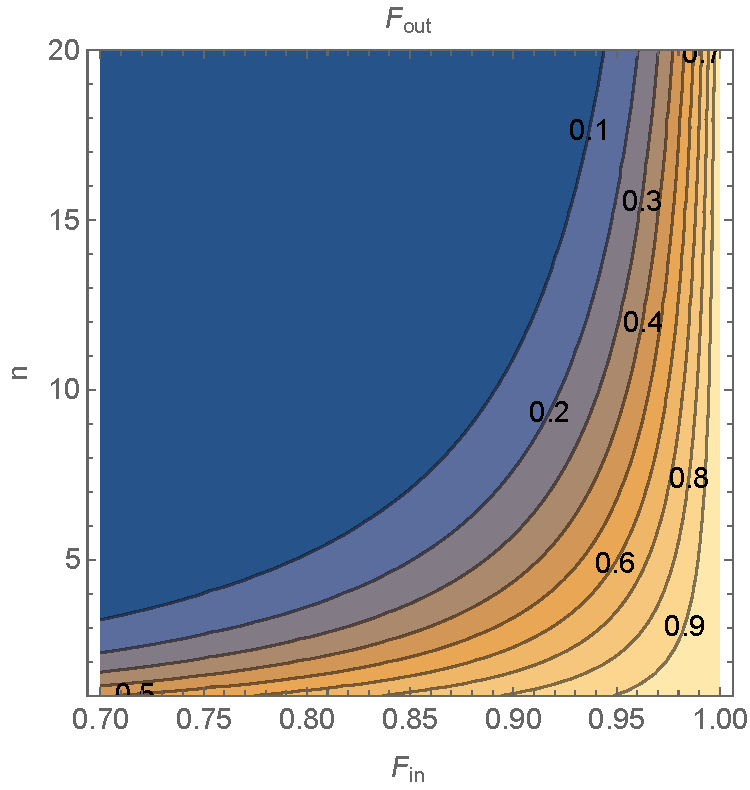
\includegraphics[width=\columnwidth]{fidelity}
\caption{Fidelity of the output state of a boson-sampler, $F_\mathrm{out}$, given single-photon input fidelities of $F_\mathrm{in}$, where $n$ is the number of photons entering the circuit.} \label{fig:fidelity}
\end{figure}

\section{Advances in Single-Photon Sources} \label{sec:adv_sources}

One of the pressing challenges facing experimental implementation of boson-sampling is SPSs. Based on the generation efficiency, single-photon sources fall into two categories: probabilistic and deterministic.

The probabilistic single-photon sources mainly includes photons created in pairs via spontaneous parametric down-conversion (SPDC) in bulk crystals \cite{bib:39, bib:40} or waveguides \cite{bib:41, bib:42}, and four-wave mixing (FWM) in waveguides \cite{bib:43, bib:44} and optical fibres \cite{bib:45, bib:46}. For these sources, the creation of photon pairs is probabilistic, rather than deterministic. However, because the photons are created in pairs, one photon (the heralding photon) can be used to herald the creation of the other photon (the heralded photon). Relatively speaking, despite being probabilistic, SPDC and FWM sources are technically mature and enjoy warm popularity in quantum optics labs. For this reason, almost all boson-sampling experiments thus far have been based on SPDC sources. 

However, SPDC or FWM might be not easily scaled to arbitrary size due to higher-order emissions, and multiplexing requirements \cite{bib:MotesScal}. Thus truly deterministic SPSs will be indispensable for future large-scale implementations. Here we only take quantum dots as an example of deterministic single-photon sources, due to their high purity, high indistinguishability, and high extraction efficiency \cite{bib:47, bib:48, bib:49, bib:50, bib:51, bib:52}. Other deterministic SPSs, such as NV centres and single atoms, are treated in excellent review papers \cite{bib:53}.

\subsection{Spontaneous Parametric Down-Conversion (SPDC)}

In SPDC, a laser pumps a second-order nonlinear material (e.g. BBO or KDP) and creates two photons under the constraints of momentum and energy conservation (known as phase-matching). There are several different types of phase matching:
\begin{itemize}
\item Type-I: Both photons have the same polarisation.
\item Type-II: Both photons have orthogonal polarisation.
\item Type-0: All polarisations are identical. \comment{How is this different to type-I?}
\end{itemize}
Additionally, so-called quasi-phase-matching in a periodically-poled structure allows a positive net flow of down-conversion, and collinear propagation direction, thus eliminating spatial walk-off effects in the transverse direction \comment{Maybe we could explain what this means? I'm a theorist and I don't know these terms :)}. As a result, the best collection efficiency of \mbox{$\sim 90\%$} is realised with quasi-phase-matching \cite{bib:41, bib:42}.

By tuning the squeezing parameter $\chi$ to approach zero, the output state may be tuned to be a vacuum state with highest probability, single photon pairs with a lower probability, and `negligible' multi-photon-pairs. As photons are produced in pairs in SPDC, one can use one photon as a trigger, and inject the other into the unitary network. Irrespective of higher-order terms and detection efficiency, the generation rate of $n$ simultaneous single-photons drops exponentially with $n$.

The best narrowband-filtered SPDC source reported thus far exhibits a purity of \mbox{$\sim 91\%$} and heralding efficiency of \mbox{$\sim 42\%$} \cite{bib:54}. Engineering the group velocity matching of crystals could help to improve the degree of spectral separability of the photons as a means to improve spectral purity \cite{bib:55, bib:56}. For a non-separable state, detection of the heralding photon collapses the state of the heralded photon onto a mixed state, i.e its spectral structure may vary between trials. With separable states, the characteristics of the heralded photon are completely independent of the measurement result obtained upon detection of the heralding photon. One such crystal is KDP, which has the property that the group velocity of e-polarised light at 415 nm is the same as that of o-polarised light at 830 nm, hence satisfying the group velocity matching conditions for separable states. These have achieved single photons with a purity of \mbox{$\sim 95\%$} and heralding efficiency \mbox{$\sim 25\%$} \cite{bib:56}. Another example is PPKTP at telecom wavelength \cite{bib:57}. More details about source engineering can be found in \cite{bib:58, bib:59, bib:60}.

\subsection{Four-Wave Mixing (FWM)}

Four-wave mixing is a third-order nonlinear effect in which two pump photons are converted into two correlated photons. Although the nonlinear effect per unit length of FWM is relatively small compared to SPDC, photon-pairs can be produced effectively by increasing the interaction length, such as in long optical fibres \cite{bib:45, bib:46} or silicon-based waveguides \cite{bib:43, bib:44}. Spontaneous Raman scattering is one of dominant noise mechanisms, however, which could be either suppressed or detuned. Recently, Spring et al. have prepared silica-based SPSs with purity \mbox{$\sim 97\%$} and heralding efficiency \mbox{$\sim 31\%$} \cite{bib:44}. They further implemented the experiments of two and three-photon Hong-Ou-Mandel interference with high visibilities \cite{bib:44}. Such heralded sources are also valuable for SBS. Another potential advantage of  FWM sources is their high coupling efficiency with circuits integrated on the same platform \cite{bib:43, bib:44}.

\subsection{Quantum Dots (QD)}

Semiconductor QDs have been researched as SPSs for a long time. Their small size (\mbox{$5\sim50$} nm) allows them to be grown via molecular beam epitaxy, resulting in a discrete energy structure for the electrons and holes, whose pairwise generation and recombination results in single-photon emission. The radiative lifetime is on the order of 1 ns. QDs can be excited either optically or electrically. Examples of optically active QDs include CdSe/ZnS, InP/GaInP, and InAs/GaAs. By embedding QDs in cavities (including planar cavities, micro-pillars, micro-disks, photonic crystals, nanowires, etc.), it has been shown that the rate of spontaneous emission can be significantly enhanced via the Purcell effect. However, it is important to note that while the generation efficiency can be close to unity, the total efficiency of the system can still be low.

Significant advances are continually emerging, enabling on-demand single-photon sources with ever increasing purity, indistinguishability and efficiency. By s-shell resonant laser excitation on a single QD with picosecond laser pulses, near-background-free resonance fluorescence (RF) has been achieved. Under $\pi$ pulse excitation, single photons have been deterministically generated with a single-photon purity of 98.8\% \cite{bib:47} and indistinguishability of 99.5\% \cite{bib:48}. Replacing the planar cavity with a micro-pillar system, RF single-photons were generated with an extraction efficiency of \mbox{$\sim 66\%$}, second-order correlation \mbox{$g_2=0.009$}, and two-photon interference visibility of 98.5\% \cite{bib:49, bib:50}. Furthermore, long streams \cite{bib:51, bib:52} of thousands of near-transform-limited single photons were measured as a function of their emission time separation varying from 13ns to 14.7. There the two-photon interference visibility slightly drops from 95.9\% to a plateau of 92.1\% through a slow dephasing process occurring at a time scale of \mbox{$0.7\mu s$} \cite{bib:51}. Currently, the only limitation is that the overall system efficiency is 4.6\% -- the highest reported in QDs. In the near future, it is hoped to improve system efficiency of quantum dot SPSs using techniques such as orthogonal excitation and detection of RF with superconducting nanowire single-photon detection.

\section{Advances in Linear Optical Networks} \label{sec:adv_networks}

Interference stability and loss are two key elements in the scalability of boson-sampling. Here we review and analyse several promising candidates for constructing linear optical networks: optical waveguides, fibre-loops, fibre beamsplitters, miniature bulk-optics, and microwave circuits.

\subsection{Optical Waveguides}

Optical waveguides are one of the most common methods to construct large-scale linear optics networks. Boson-sampling was also first demonstrated mainly using this technology \cite{bib:4, bib:5, bib:6}. Compared to discrete bulk-optical elements, waveguides can be integrated onto a small chip, which is free of alignment, more compact, and phase-stable. The main obstacle facing scaling up waveguide platforms is their high loss, including propagation loss, and coupling loss between waveguides and the photon sources/detectors. Here we discuss several of them briefly.

The first waveguide platform we consider is silica-on-silicon planar lightwave circuits (PLC) \cite{bib:61}, due to its ultra-low propagation loss ($<0.01$dB/cm) and coupling loss ($<0.1$dB/facet). In present small-scale quantum applications \cite{bib:9}, its coupling loss of $\sim 0.4$dB/facet may be low enough. However, each directional coupler (DC) exhibits loss of $\sim 0.1$dB, still unacceptable for large-scale circuits containing hundreds of DCs. In principle, losses could be improved to meet requirements using state-of-the-art techniques. Another more severe problem dimming the prospect for such micrometer waveguides is the size of DCs. As shown in Tab.~\ref{tab:one}, the smallest radius is 2mm, achieved by PLC waveguides with index contrast of 1.5\%, allowing for tight bends and shortest DC length (1mm). In fact, they usually reach several millimetres \cite{bib:9}, leading to an exaggerated total length of $\sim 1$m for circuits containing hundreds of DCs.

\begin{table*}
\begin{tabular}{|c|c|c|c|c|c|}
\hline
Silica & Technology & $\Delta$(\%) & Min. radius (mm) & PL (db/cm) & CL (dB/facet) \\
\hline
\hline
Ge-doped & PLC  & 0.25 & 25 & $<0.01$ & $<0.1$ \\
Ge-doped & PLC  & 1.5  & 2  & 0.05    & 2.0 \\
Fused    & FLDW & 0.7  & 50 & 0.3     & 0.1 \\
Fused    & FLDW & 1.0  & 15 & 0.6     & 0.1 \\
\hline
\end{tabular} \caption{Properties of waveguides fabricated by PLC \cite{bib:61} and FLDW \cite{bib:62} (wavelength: 1550 nm).} \label{tab:one}
\end{table*}

The problem of size also haunts another popular platform in the field of optical quantum processing -- fused silica waveguides, fabricated using femtosecond laser direct-written (FLDW) technology. Unlike PLC fabrication, the FLDW is a powerful and flexible technique for rapid 3D fabrication, requiring no masking procedure or cleanroom environment. However, this one-step fabrication process also makes the propagation loss rely heavily on the motion control accuracy of the precision stage \cite{bib:63}. FLDW waveguides exhibit lowest losses on the order of 0.1dB/cm \cite{bib:63}, substantially higher than that of PLC waveguides. Also, the maximum refractive index contrast achieved so far is 1\%, which limits waveguide bends to a radius of about 15 mm (see Tab.~\ref{tab:one}).

A possible solution to relaxing this problem is silicon nitride ($\mathrm{Si}_3\mathrm{N}_4$) planar waveguides, which are also transparent from visible through telecom wavelengths. Thanks to higher refractive index contrast ($\sim 25$\%), their integration density could be about an order of magnitude more compact than silica waveguides. In fact, Bowers et al. have developed high-aspect-ratio $\mathrm{Si}_3\mathrm{N}_4$ waveguides with favourably low propagation loss ($<1$dB/m) \cite{bib:64}, and minimum bend radii less than 1mm \cite{bib:65}.

Another possible solution would be silicon waveguides, which have higher refractive index than the other waveguides mentioned previously, thus allowing a dramatic reduction in the bend radius ($<10\mu\mathrm{m}$). Correspondingly, the length of DC can be dramatically reduced, e.g. the $2\times 2$ MMI coupler in silicon ($27\mu\mathrm{m}$) \cite{bib:66} is 40 times shorter than the one in silica (1.1mm) \cite{bib:67}. On the other hand, the best propagation losses can reach 0.1dB/cm \cite{bib:68, bib:69} and coupling losses of 0.5dB/facet are possible using spot-size converters (SSC) \cite{bib:70, bib:71}. That is to say, it is possible to construct large networks with thousands of DCs with insertion loss as low as 2dB in principle. However, current quantum experiments based on silicon waveguides \cite{bib:43, bib:72} have typical propagation losses of $2\sim 4$dB/cm and coupling losses of $2\sim 4$dB/facet, leading to device losses in the range of $6\sim 10$dB. Another important loss we cannot ignore is the excess loss of each DC, on the order of 0.1dB \cite{bib:72, bib:73, bib:74}, a substantial hurdle in the quest for scalability. Note that visible wavelengths, including 780nm, are forbidden, but 1550nm, the typical telecom wavelength, is in its transparent window and can be detected with high-efficiency ($>95\%$) using superconducting single-photon detectors \cite{bib:75}.

\subsection{Fibre-Loops}

The fibre-loop architecture \cite{bib:11, bib:19}, where a pulse-train of time-bin-encoded photons are employed, is extremely resource-frugal, irrespective of the size of the desired interferometer, whose scale is limited only by the loss rates of the fibre, dynamic switches and couplers. The scheme requires only two delay lines, three dynamic switches, a single photon source operating at high repetition rate, and a single time-resolved photodetector. The architecture is shown in Fig.~\ref{fig:loop_arch}.

Depending on the scale of the time-bins, the fibre loops could be replaced by any delay lines, or even propagation in free-space, which would eliminate fibre loss. In this case, the dominant source of loss would be in the dynamic switches and couplers. While state-of-the-art integrated switches/couplers are fast enough, on the order of GHz \cite{bib:76, bib:77}, they involve high loss ($>1$dB). This will encourage further development of these types of technologies.

In order to lower loss \cite{bib:11}, the controlled switch was realised using a bulk electro-optic modulator (EOM) with a transmission ratio of 97.3\%, modulated at 80MHz. The single-photons were coupled in and out of the loop using an acousto-optic modulator (AOM) with a transmission ratio of 99\%, rise-time of less than 20ns and first order diffraction efficiency of $\sim 85\%$. Inside the loop, the coupling efficiency from free-space to single-mode fibre was 92\%. Thus, a single-loop (BS operation) efficiency of 83\% was achieved.

\subsection{Fibre Beamsplitters}

Due to the ultra-low loss of single mode fibres (0.2dB/km at 1550nm), fused fibre couplers (FFC) are a promising candidate. The couplings between any two adjacent fibres are hard to control on a large scale due to the fusing process, thus commercial FFCs are rare with greater than $4\times 4$ input/output modes. In fact, such random coupling devices are not welcomed by applications other than boson-sampling. In one of the first demonstrations of boson-sampling \cite{bib:10}, the circuit was a 3�3 FFC with coupling efficiency of 64\%. Recently, Lin et al. \cite{bib:78} fabricated a $15\times 15$-mode FBS and claimed that such a large-scale device has a total loss as low as 1dB, and could potentially be scaled up to hundreds of modes with improvements to the fabrication process.

\subsection{Miniaturised Bulk-Optics}

As mentioned above, discrete bulk-optics circuits exhibit unacceptable physical size and phase-stability problems. However, all the optical elements can be antireflection-coated easily and with near-perfect transmission ratios ($>99.9\%$). For this reason bulk-optics should nonetheless be considered a good candidate for the implementation of linear optical networks, provided some necessary technological improvements. If one could miniaturise the size of each element down to the $\sim 1$mm scale, a 20-photon boson-sampling circuit would only cover an area of less than $1\mathrm{m}^2$, which would fit on a standard optical table. In order to solve the phase-stability problem, all elements could be bonded together using the optical contact technique or placed into a constant temperature vacuum chamber.

\subsection{Microwave Circuits}

In microwave boson-sampling, to guarantee that all operations finish before photons escape the cavity, the total operational time must be less than the cavity lifetime. With present-day technology ($150\mu\mathrm{s}$ cavity lifetime), we are able to scale microwave boson-sampling to 500 modes. As demonstrated in \cite{bib:20}, present superconducting technology has the ability to scale microwave boson-sampling to $N\sim 20$. Supposing a total efficiency of 0.65 (0.99 fidelity for each step, and in total 20 steps for each mode, then multiplying the preparation and measurement efficiency $0.9\times 0.9$), a conservative estimate would be that 20-photon microwave boson-sampling could match the performance of a classical computer of gigaFLOPS, beyond our expectation for ordinary optical boson-samplers with today's technology. 

On the other hand, microwave boson-sampling is also suitable for generalised versions of boson-sampling, e.g. boson-sampling using cat states \cite{bib:79}, photon-added or photon-subtracted squeezed states \cite{bib:80}, displaced single-photon Fock states and single-photon-added coherent states \cite{bib:81}, and molecular vibronic spectra \cite{bib:82}. Arbitrary quantum states have already been synthesised in superconducting resonators with an average fidelity of 0.9 \cite{bib:83}. Furthermore, photon-number-resolving measurement has been described using several methods \cite{bib:84, bib:85}.

\section{Advances in Single-Photon Detectors} \label{sec:adv_detectors}

Last but not least, we briefly discuss single-photon detectors, the final and very important stage in the experimental implementation of boson-sampling. Single-photon detectors with high quantum efficiency, low dark-noise and fast response are a pressing goal to scale up boson-sampling to the post-classical scale. There are a variety of single-photon detectors, detailed descriptions of which can be found in several excellent review papers \cite{bib:53, bib:86}. Targeting the most widely used single-photon sources in boson-sampling experiments, probabilistic SPDC sources and deterministic single-photons from quantum dots \cite{bib:11}, as well as emerging on-chip sources based on semiconductor devices \cite{bib:43, bib:44}, we mainly focus on single-photon detectors that have good spectral response in the near-infrared region ($780\sim 1550$nm), the typical wavelength of such photon sources.

\subsection{Single-Photon Avalanche Diodes (SPAD)}

Firstly, the most compact and common single-photon detector is the single-photon avalanche diode (SPAD). SPADs are avalanche diodes operated in Geiger mode (above breakdown voltage) to obtain a high gain. To our knowledge, there are several SPADs available commercially off-the-shelf, with detection efficiencies around 60\% at 780nm, maximum count-rates of 25MHz and dark-count rates as low as 25Hz. Even higher detection efficiencies are available. However, on account of the significant trade-off between detection efficiency, dark-noise and dead-time (affected by after-pulsing effects), it is often at the expense of a lower maximum count rate (a typical dead-time is $1\mu\mathrm{s}$, yielding a 1MHz count rate) and higher levels of dark-noise. It should be noted that the features of detectors are usually optimised at different wavelengths according to specific needs.

\subsection{Superconducting Nanowire Single-Photon Detectors (SNSPD)}

More efficient are superconducting nanowire single photon detectors (SNSPD). Up until now, the highest detection efficiency of SNSPDs is 93\% at 1550nm, demonstrated in 2014 \cite{bib:87}. SNSPDs are also commercially available. There are companies specialising in best-performance SNSPDs with high detection efficiency. They have achieved specifications with peak detection efficiencies higher than 80\% around 800nm, maximum dark-count rates of $100\sim 300$Hz, and a dead-time ranging from $10\sim 70$ns. Similar performance is expected for optimised SNSPD at other wavelengths ($780\sim 1550$nm). However, SNSPDs must be operated at cryogenic temperatures of a few Kelvin to maintain the superconducting state in the sensing material. This is the main reason why SNSPDs are much more cumbersome and expensive than SPADs.

\subsection{Superconducting Transition-Edge Sensors (TES)}

Titanium superconducting transition edge sensors (TES), exploit the character that the resistance of a superconducting material increases sharply and linearly when its temperature surpasses the superconducting critical temperature. Using such detectors, even higher detection efficiencies of 98\% (95\%) at wavelengths around 850nm (1556nm) have been reported \cite{bib:88, bib:75}. Moreover, these detectors are photon-number-resolving, owing to the linear relationship between resistance and temperature. TESs far outperforms other kinds of single-photon detectors in many important respects: high detection efficiency; photon-number resolution; and, low dark-noise. However, the typical thermal recovery times of TESs are a fraction of a microsecond, resulting in low count rates and limiting their application in quantum simulation. The superconducting transition temperature of titanium is in the range of 100mK, more than an order of magnitude lower than SNSPD, which makes it challenging to migrate the technique from lab to market. On the other hand, higher superconducting transition temperatures are also favourable for faster recovery times. Thus, high temperature superconductors will have great implications for future single-photon detectors.

In summary, for state-of-the-art single-photon detectors, high performance detectors are available, but not sufficient with respect to the three key detector features of relevance to boson-sampling, and the challenging optimisations given the interplay between the different parameters.

\section{Conclusion} \label{sec:conclusion}

We constructed a rigorous and fair model for comparing the performance of genuine boson-samplers with classical simulators by taking both the repeat frequency and system efficiency of the boson-sampling system into account. We also considered the effects of error models such as mode-mismatch, photon distinguishability, spectral impurity and time-jitter, and how these relate to the size of the boson-sampler.

In our model, we can easily determine how many single-photons, and what repeat frequency and efficiency are needed to beat classical computers with given clock-speeds. To attain quantum supremacy, there are lower single-photon number thresholds ($<20$ photons) in systems with higher efficiencies and repeat frequencies. Therefore, improving repeat frequency plays a bigger role than photon number for those circuits with limited size but high transmittance, e.g., bulk optical circuits. \comment{Don't quite understand this last sentence}.

From the asymptotic flavour of computational complexity, implementing boson-sampling with more single-photons would be of interest to theorists. It is crucial to improve efficiencies of every part of the system, which is the dominant effect undermining sampling rates as photon-number increases.

In the latter half of this paper, we reviewed and clarified the advantages and disadvantages of different protocols and systems, including single-photon sources, optical circuits and single-photon detectors, which will shed light the road towards scalability of boson-sampling experiments. Among the different combinations, scattershot boson-sampling and normal boson-sampling with quantum dots are the two most promising routes forward. In order to realise larger scale boson-sampling ($>20$ photons), however, the former still requires improving the heralding efficiency of SPDC photon sources, while the latter requires developing either ultra-high efficiency delay-loops or active multiplexing techniques \cite{bib:89}. Both must further lower circuit losses if the elusive goal of demonstrating quantum supremacy is to be achieved.

The analysis presented here provides an initial roadmap for what is perhaps the most promising route towards the first demonstration of quantum supremacy over classical computers. While we have focused largely on experimental issues surrounding the implementation of boson-sampling, there remain significant theoretical challenges facing large-scale realisations. Most notably, verification of boson-sampling data has shown itself to be a highly non-trivial problem. To-date, no unambiguous test has been described for verifying the validity of boson-sampling data. Significant progress has been made in processing experimental data to rule out some classical theories, such as uniform sampling and distinguishable photon sampling, but proving categorically that a sample set originated from a genuine boson-sampler remains an unsolved problem. It may very well never be solved, as many quantum algorithms are believed to not be efficiently verifiable. Quite plausibly, boson-sampling is one of them.

Also from a theoretical perspective, is the broader question of `What good is a boson-sampler? What does it even do?'. The answer is that, to the best of our knowledge, it really doesn't solve any particular problem of practical interest, which may lead some to question the merit of pursuing this line of research at all. However, we take the entirely opposing view that, although it doesn't solve a problem of interest, the mere fact that it could outperform existing classical computers and provide a proof-of-principle of quantum supremacy would already be a stunning achievement. And given the relative simplicity of the boson-sampling architecture, and the rapid developments taking place in the field, it is plausible that the first ever post-classical quantum device may be a boson-sampler.

%
% Acknowledgments
%

\begin{acknowledgments}
\end{acknowledgments}

\appendix

\section{Numerically Modelling the Effects of Signal-to-Noise Ratios}

\section{Details of Scattershot Boson-Sampling Analysis}

%
% Bibliography
%

\bibliography{roadmap}

\end{document}
